\documentclass[12pt]{article}
\usepackage[T1]{fontenc}
\usepackage[T1]{polski}
\usepackage[utf8]{inputenc}
\usepackage{graphicx}
\usepackage{amsfonts}
\usepackage{float}

\setlength{\textheight}{20cm}

\title{{\bf Zadanie nr 4 -Przekształcenie Fouriera, Walsha-Hadamarda, kosinusowe i falkowe,
szybkie algorytmy.}\linebreak
Cyfrowe Przetwarzanie Sygnałów}
\author{Krzysztof Barden, 210139 \and Paweł Galewicz, 210182}
\date{14.06.2019r.}

\begin{document}
\clearpage\maketitle
\thispagestyle{empty}
\newpage
\setcounter{page}{1}
\section{Cel zadania}

Celem ćwiczenia jest zapoznanie się z operacjami transformacji sygnałów dyskretnych
przy użyciu wybranych metod.



\section{Wstęp teoretyczny}

Program z zadania 1 ,2  i 3 został rozszerzony o dodadtkowe funkcjonalnosci. Wykresy generowane są przy użyciu biblioteki LiveCharts \cite{lv}. GUI aplikacji zostało stworzone przy użyciu biblioteki WPF \cite{wpf}.
\\Interfejs generacji sygnałów został rozszerzony o możliwosć generacji dodatkowego sygnału o następującym wzorze:
\begin{figure}[H]
 \centering
 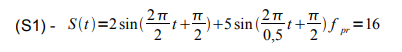
\includegraphics[width=15cm]{images/signal.PNG}
 \vspace{-0.3cm}
 \caption{Wzór sygnału S1}
 \label{gui}
\end{figure}
\begin{figure}[H]
 \centering
 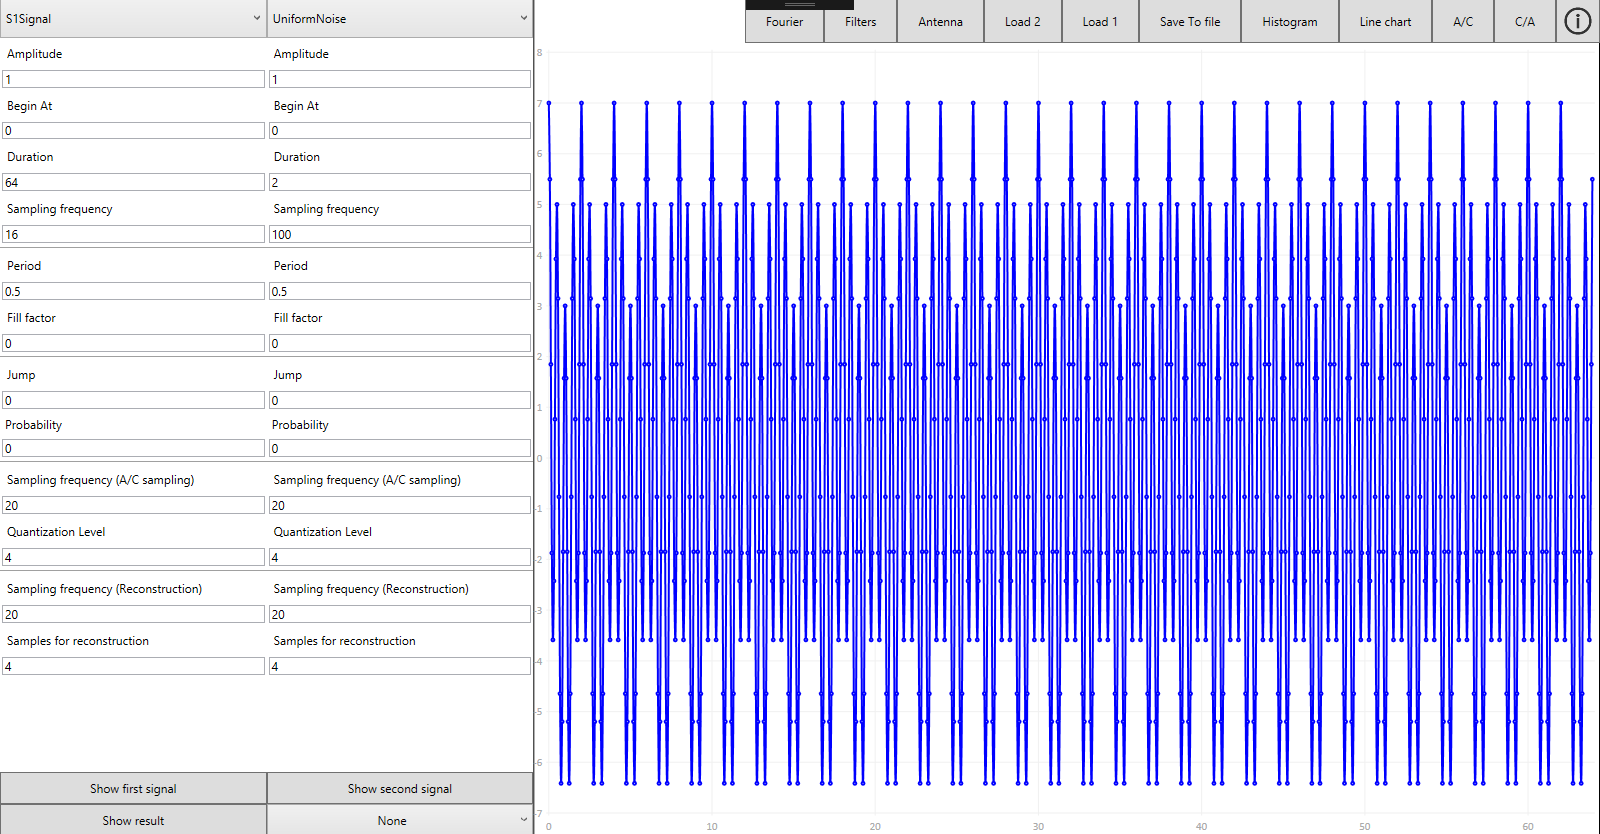
\includegraphics[width=15cm]{images/newsignal.PNG}
 \vspace{-0.3cm}
 \caption{Wygenerowany sygnał S1}
 \label{gui}
\end{figure}
Do programu został dodany interfejs z operacjami transformacji:
\begin{figure}[H]
 \centering
 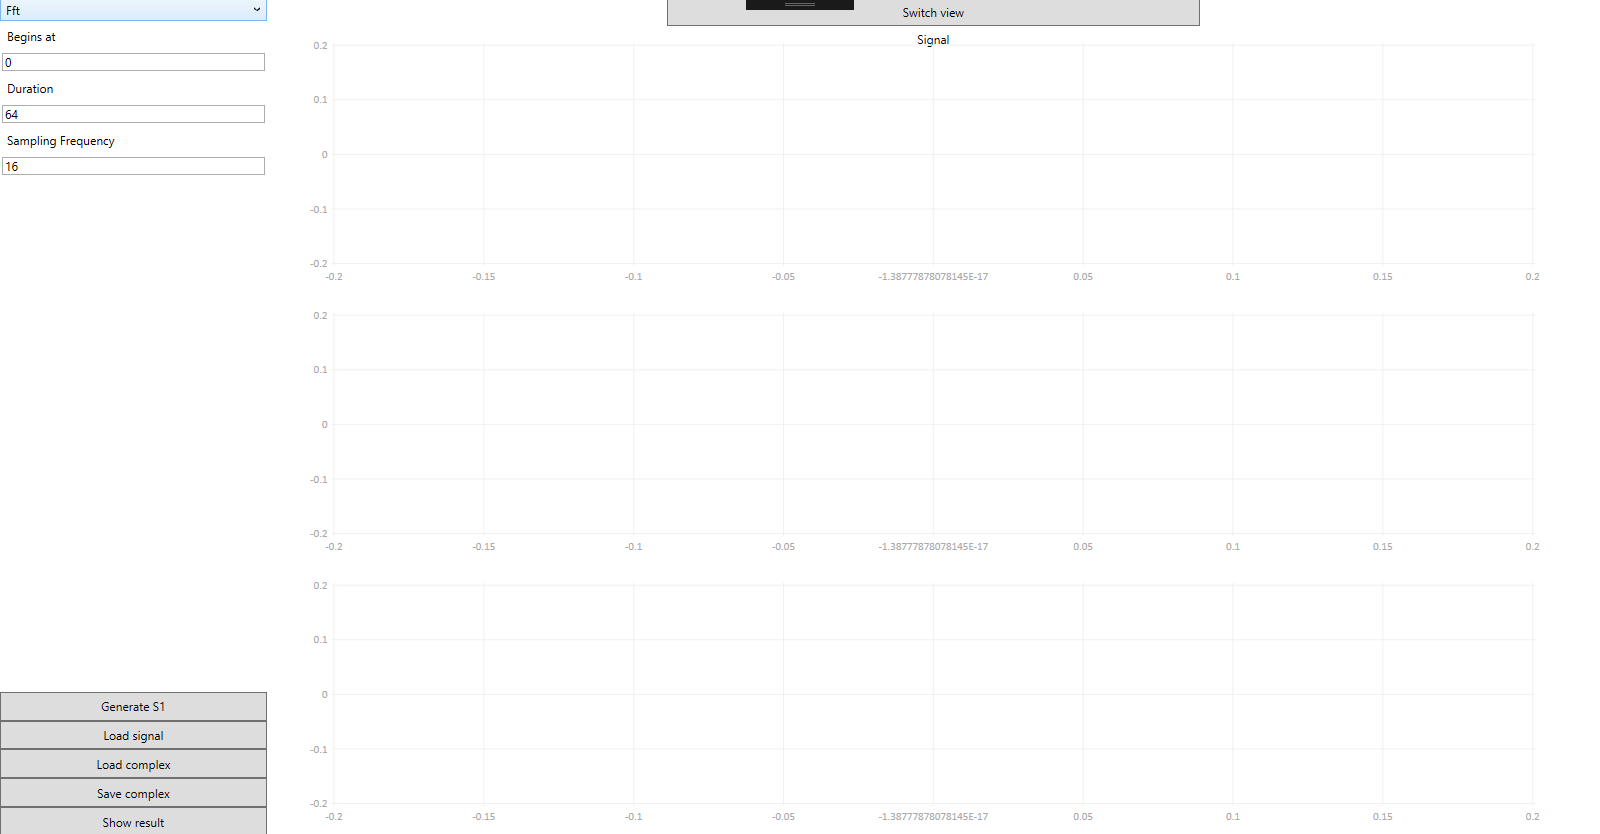
\includegraphics[width=15cm]{images/fourierWindow.PNG}
 \vspace{-0.3cm}
 \caption{Interfejs graficzny operacji transformacji}
 \label{gui}
\end{figure}

Pierwszy wykres jest wykresem sygnału transformowanego.
Możliwe są dwa tryby prezentacji wykresów. 
\begin{itemize}
\item (W1) – górny wykres prezentuje część rzeczywistą amplitudy w funkcji
częstotliwości, a wykres dolny część urojoną;
\item (W2) – górny wykres prezentuje moduł liczby zespolonej, a dolny argument liczby
w funkcji częstotliwości.
 splotu.
\end{itemize}
Zaimplementowane zostały następujące tranformacje sygnałów:
\begin{itemize}
\item (F1) – dyskretna transformacja Fouriera – algorytm z definicji oraz szybka
transformacja Fouriera z decymacją w dziedzinie czasu (DIT FFT)
\item (T1) – transformacja kosinusowa typu drugiego (DCT II) oraz szybka transformacja
kosinusowa (FCT II)
\end{itemize}

Interfejs ten pozwala na zapisanie sygnału transformowanego, zapisanie i wczytanie sygnału w postaci zespolonej. Górny przycisk pozwala na przęłączenie pomiędzy trybami prezentacji wykresów.
\section{Eksperymenty i wyniki}


%%%%%%%%%%%%%%%%%%%%%%%%%%%%%%%%%%%%%%%%%%%%%%%%%%%%%%%%%%%%%%%%%%%%%%%%%%%%%%%%%%%%%%%%%%%%%%%%%%%%%%%%%%%%%%%%%
% PODROZDZIAŁ PT. EKSPERYMENT NR 1 
%%%%%%%%%%%%%%%%%%%%%%%%%%%%%%%%%%%%%%%%%%%%%%%%%%%%%%%%%%%%%%%%%%%%%%%%%%%%%%%%%%%%%%%%%%%%%%%%%%%%%%%%%%%%%%%%%

\subsection{Eksperyment nr 1 }
\subsubsection{Dyskretna transformacja Fouriera}
Celem tego eksperymentu zaprezentowanie możliwosci programu do wykonania dyskretnej transformacji Fouriera.
Czas wykonania operacji: 157ms.

\subsubsection{Rezultat}
\begin{figure}[H]
 \centering
 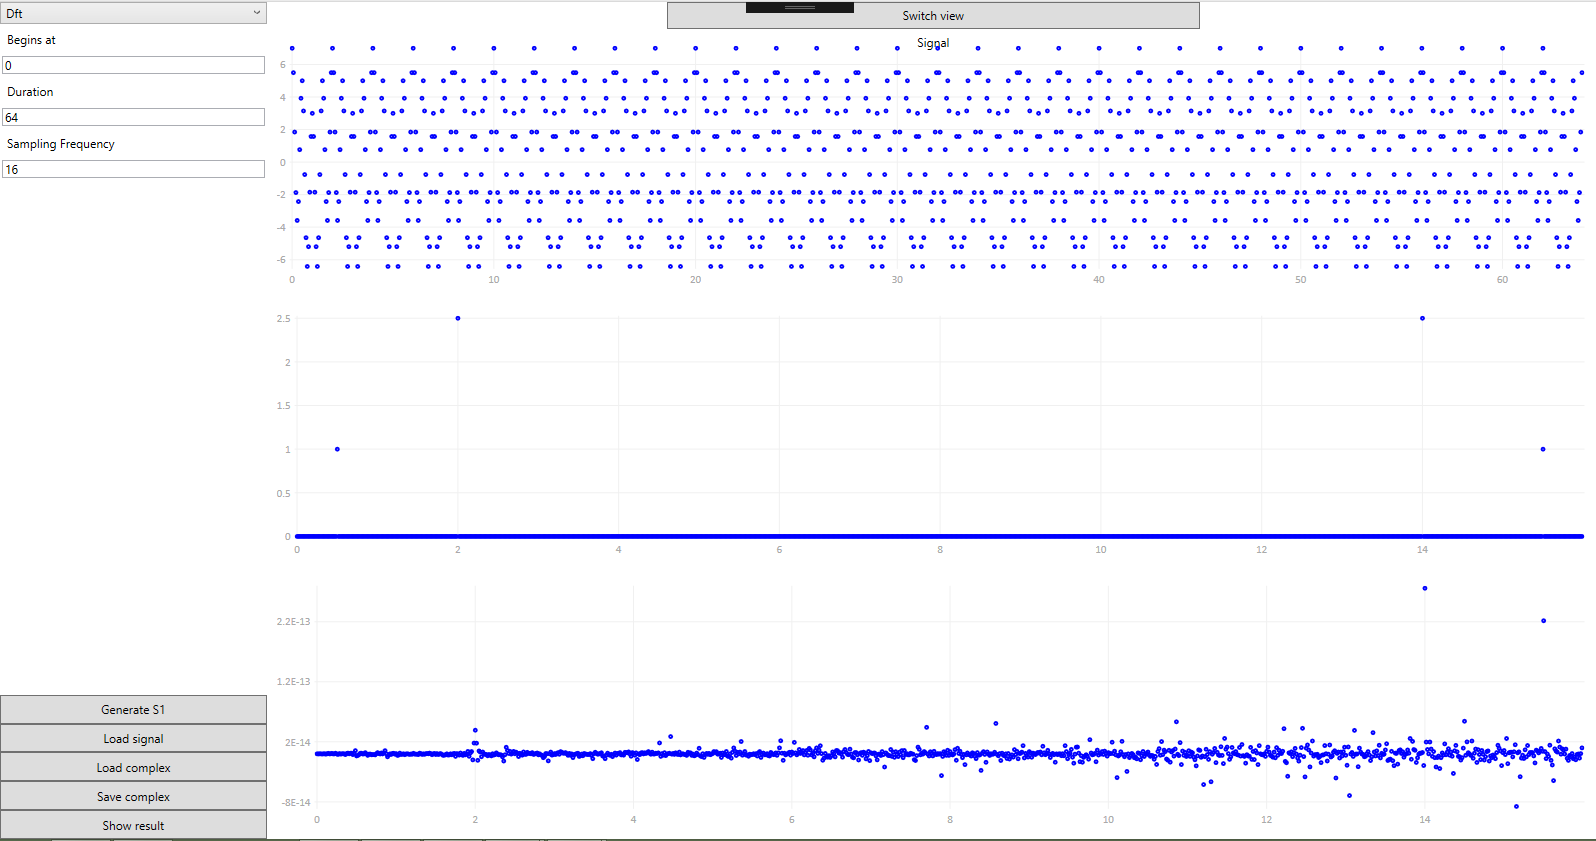
\includegraphics[width=14cm]{images/dftw1.PNG}
 \vspace{-0.3cm}
 \caption{DFT W1}
 \label{gui}
\end{figure}
\begin{figure}[H]
 \centering
 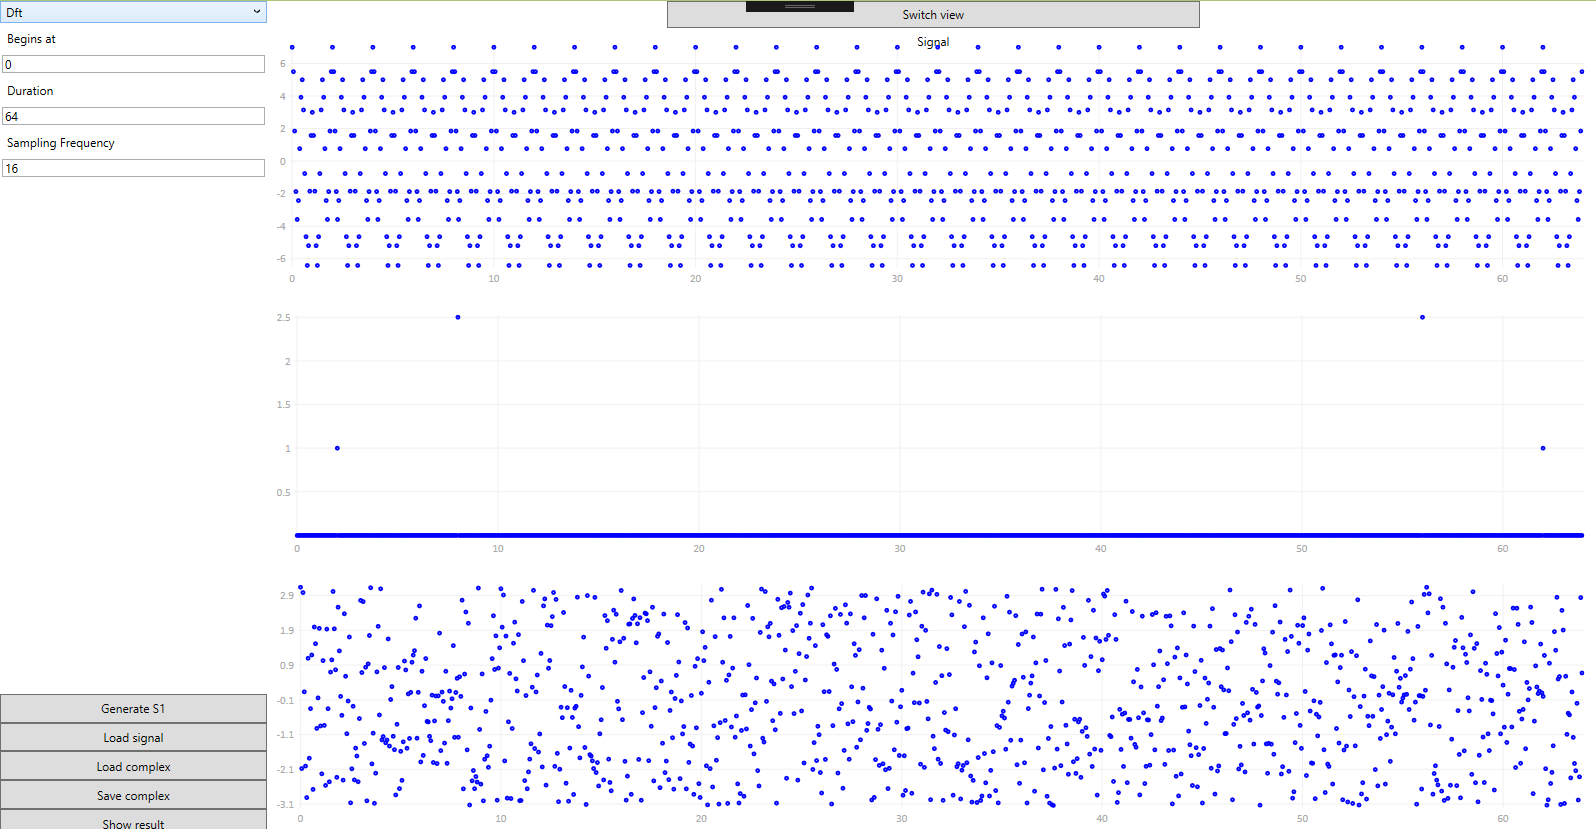
\includegraphics[width=14cm]{images/dftw2.PNG}
 \vspace{-0.3cm}
 \caption{DFT W2}
 \label{gui}
\end{figure}

%%%%%%%%%%%%%%%%%%%%%%%%%%%%%%%%%%%%%%%%%%%%%%%%%%%%%%%%%%%%%%%%%%%%%%%%%%%%%%%%%%%%%%%%%%%%%%%%%%%%%%%%%%%%%%%%%
% PODROZDZIAŁ PT. EKSPERYMENT NR 2
%%%%%%%%%%%%%%%%%%%%%%%%%%%%%%%%%%%%%%%%%%%%%%%%%%%%%%%%%%%%%%%%%%%%%%%%%%%%%%%%%%%%%%%%%%%%%%%%%%%%%%%%%%%%%%%%%

\subsection{Eksperyment nr 2 }
\subsubsection{Szybka transformacja Fouriera  z decymacją w dziedzinie czasu}
Celem tego eksperymentu zaprezentowanie możliwosci programu do wykonania szybkiej transformacji Fouriera z decymacją w dziedzinie czasu.
Czas wykonania operacji: 33ms.

\subsubsection{Rezultat}
\begin{figure}[H]
 \centering
 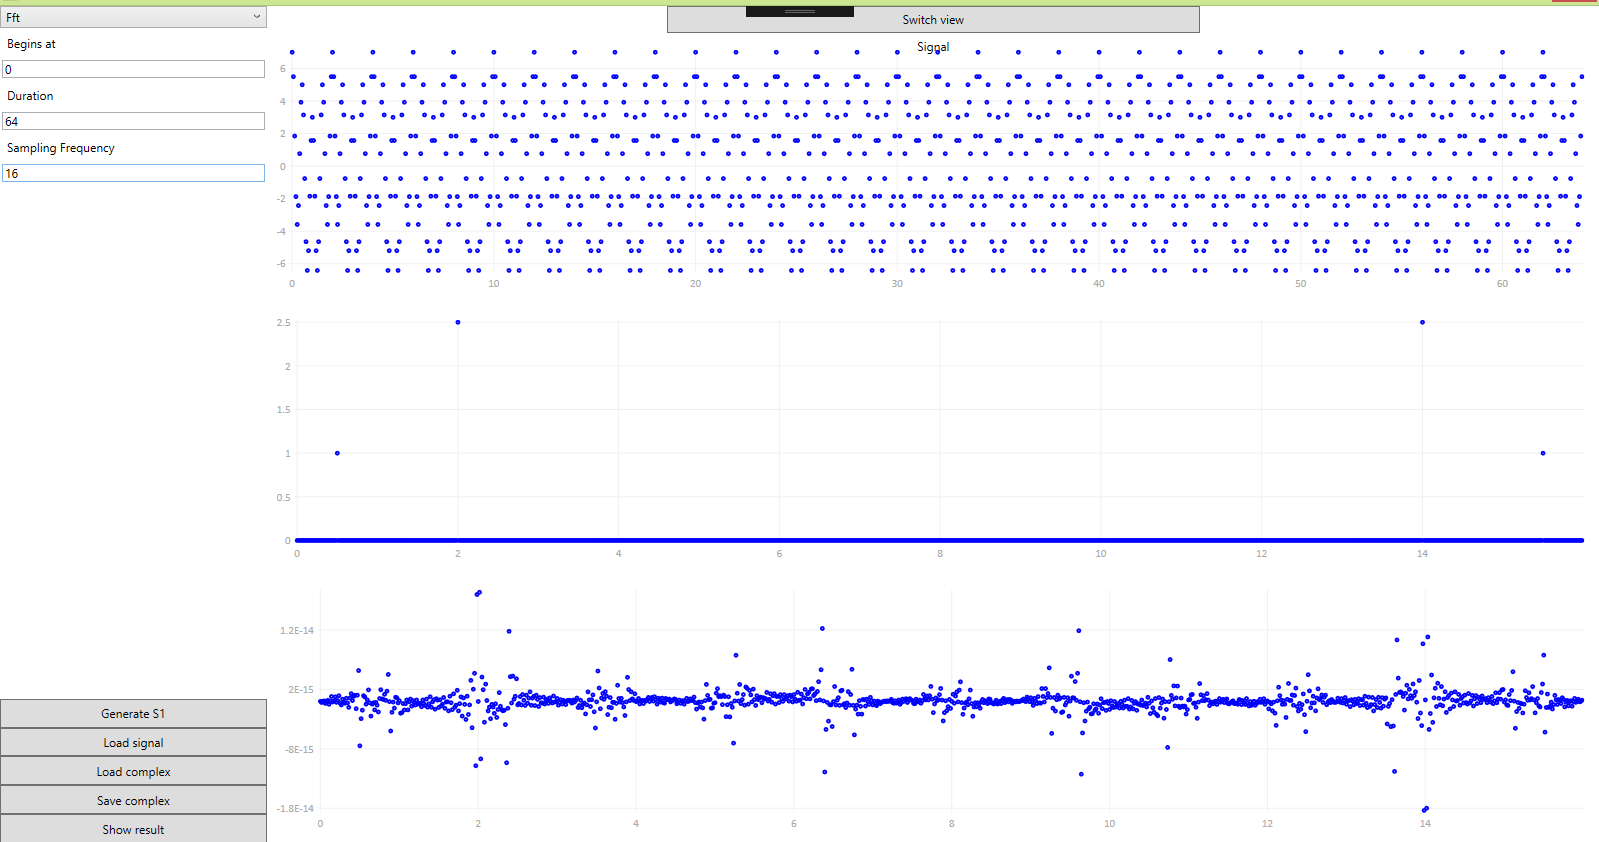
\includegraphics[width=14cm]{images/fftw1.PNG}
 \vspace{-0.3cm}
 \caption{FFT W1}
 \label{gui}
\end{figure}
\begin{figure}[H]
 \centering
 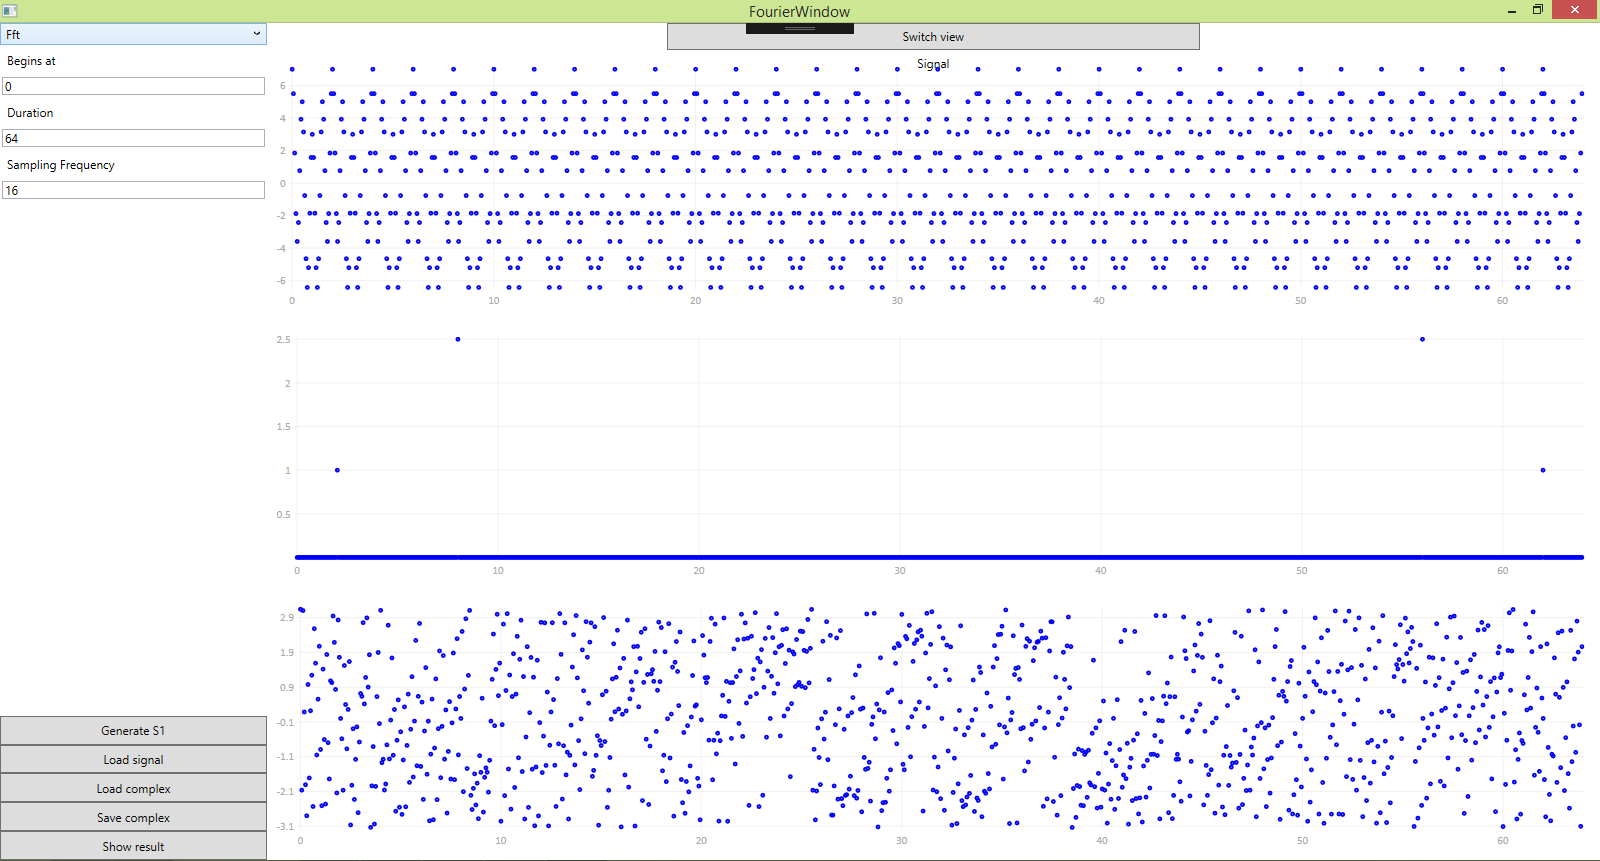
\includegraphics[width=14cm]{images/fftw2.PNG}
 \vspace{-0.3cm}
 \caption{FFT W2}
 \label{gui}
\end{figure}





%%%%%%%%%%%%%%%%%%%%%%%%%%%%%%%%%%%%%%%%%%%%%%%%%%%%%%%%%%%%%%%%%%%%%%%%%%%%%%%%%%%%%%%%%%%%%%%%%%%%%%%%%%%%%%%%%
% PODROZDZIAŁ PT. EKSPERYMENT NR 3
%%%%%%%%%%%%%%%%%%%%%%%%%%%%%%%%%%%%%%%%%%%%%%%%%%%%%%%%%%%%%%%%%%%%%%%%%%%%%%%%%%%%%%%%%%%%%%%%%%%%%%%%%%%%%%%%%




\subsection{Eksperyment nr 3 }
\subsubsection{Korelacyjny czujnik odległosci}
Do zaprezentowania możliwosci korelacyjnego czujnika odległosci przedstawimy eksperyment w którym dokonamy pomiarów dla 3 sygnałów, każdy z innymi parametrami sygnałów.


\subsubsection{Rezultat}

\begin{figure}[H]
 \centering
 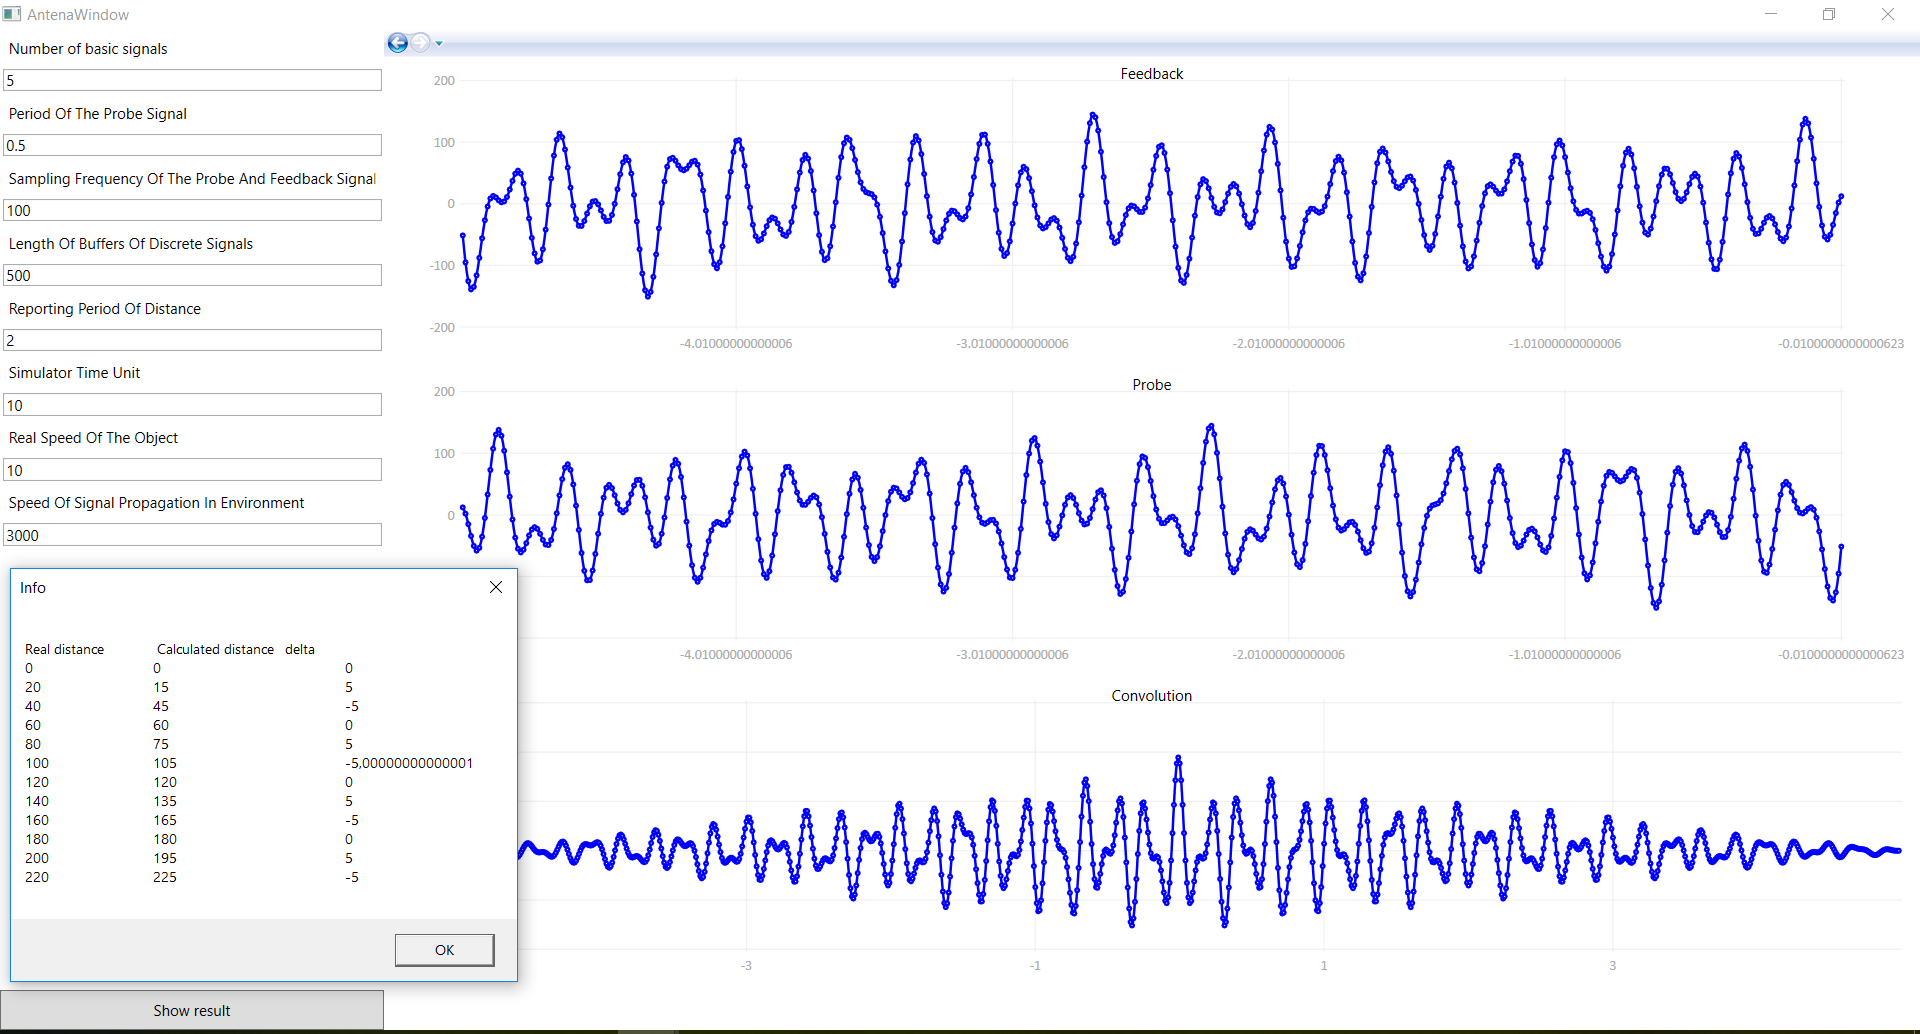
\includegraphics[width=14cm]{images/a1.PNG}
 \vspace{-0.3cm}
 \caption{Korelacyjny czujnik odległosci}
 \label{gui}
\end{figure}

\begin{figure}[H]
 \centering
 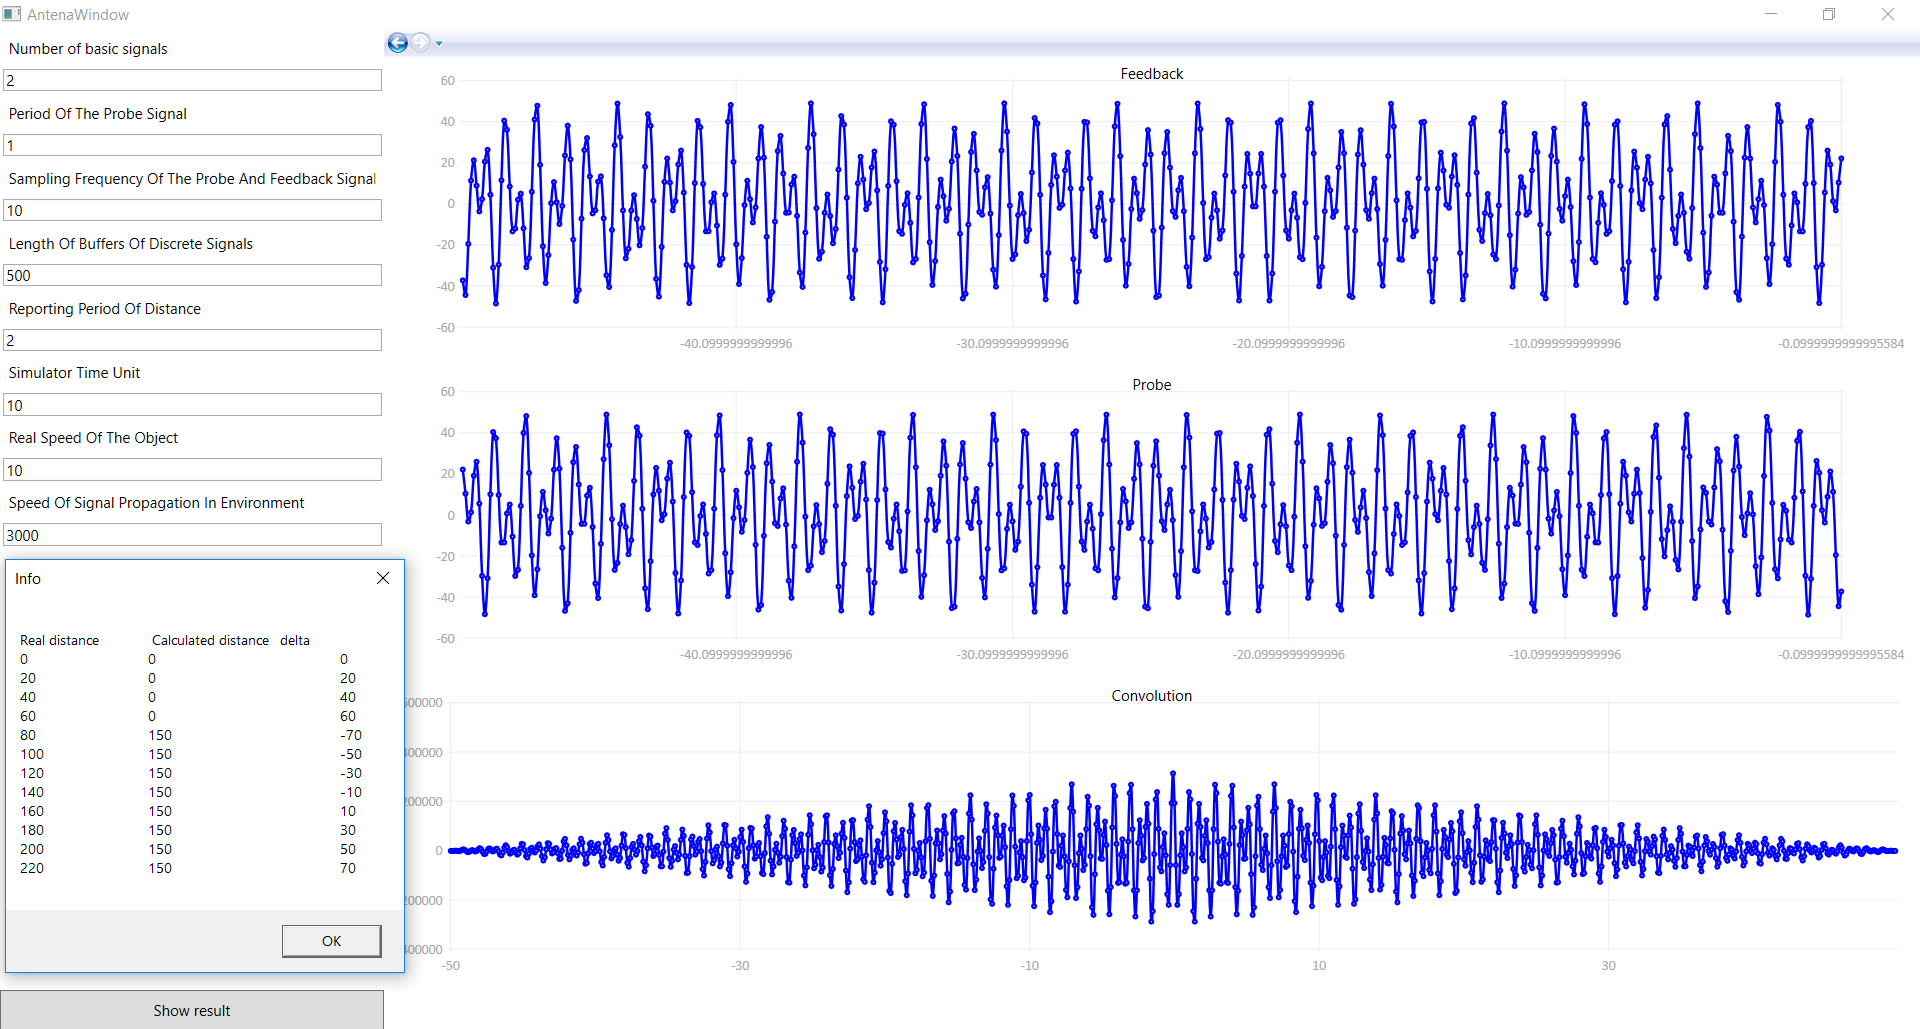
\includegraphics[width=14cm]{images/a2.PNG}
 \vspace{-0.3cm}
 \caption{Korelacyjny czujnik odległosci}
 \label{gui}
\end{figure}


\begin{figure}[H]
 \centering
 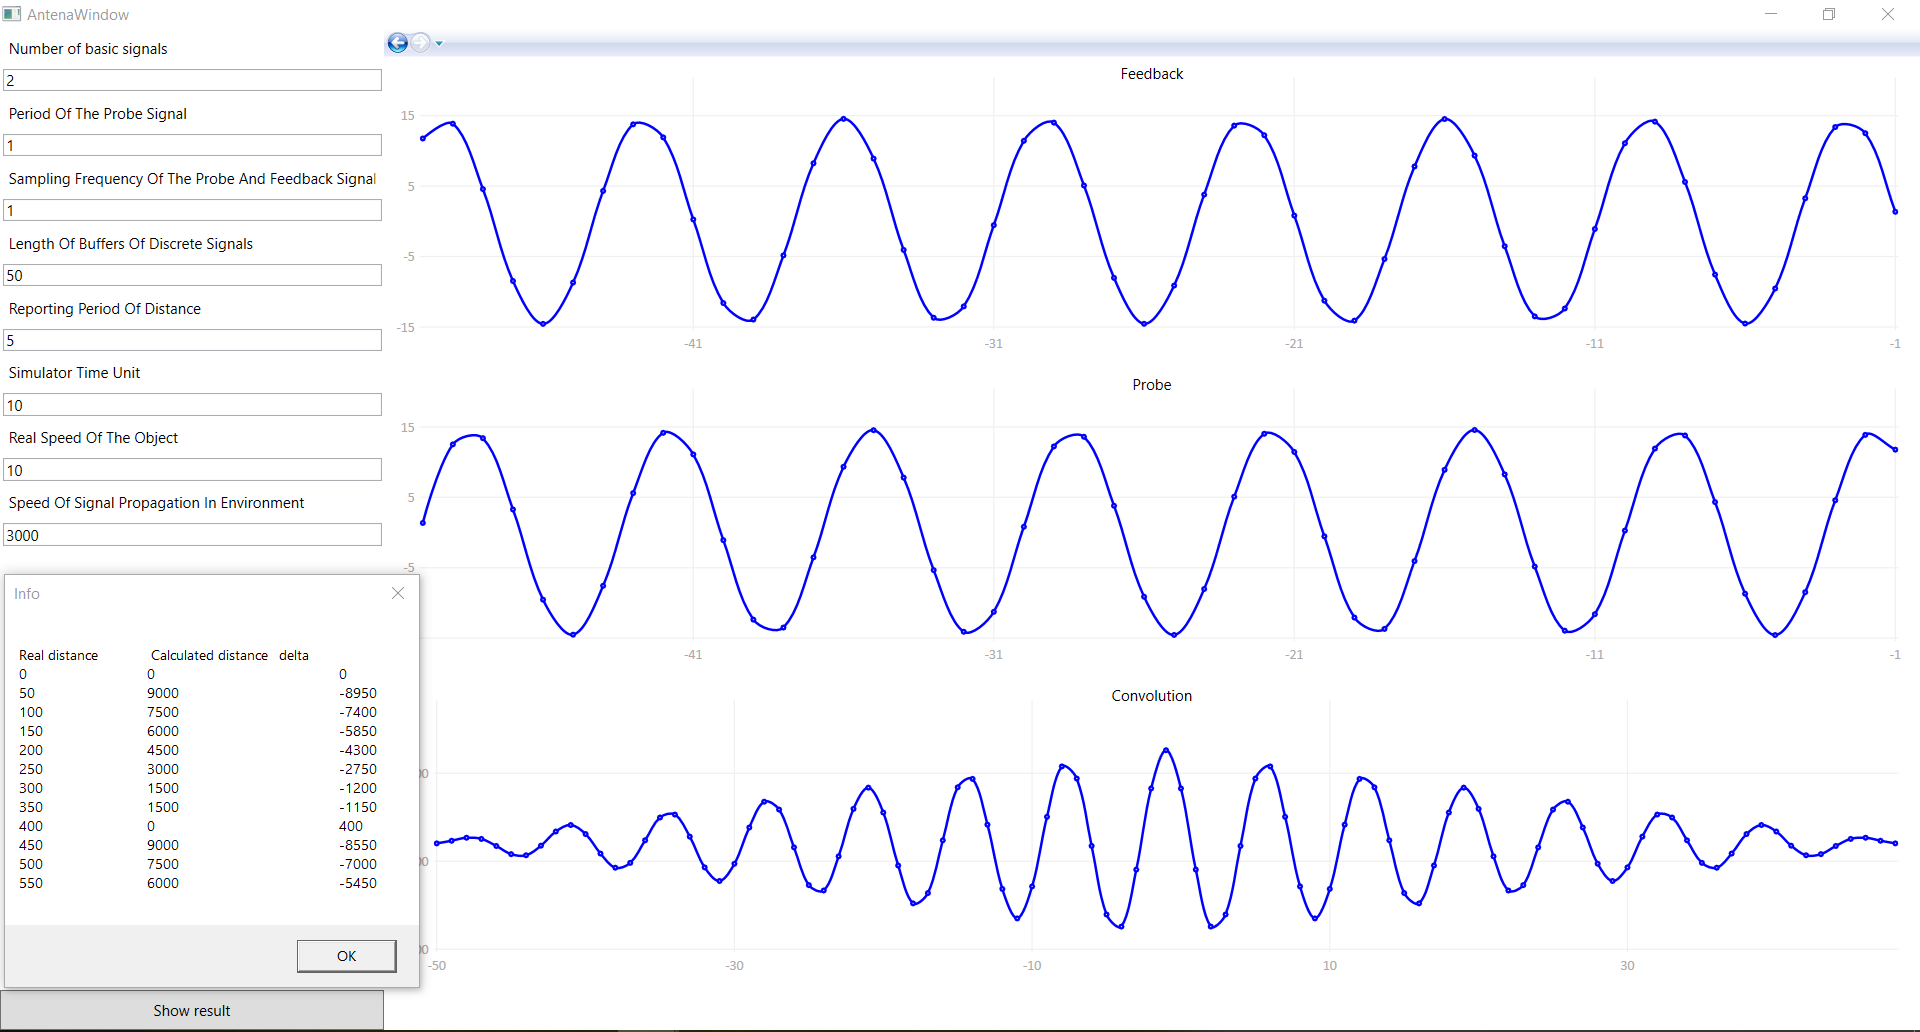
\includegraphics[width=14cm]{images/a3.PNG}
 \vspace{-0.3cm}
 \caption{Korelacyjny czujnik odległosci}
 \label{gui}
\end{figure}


\newpage

\section{Wnioski}

Aplikacja została napisania zgodnie z instrukcją zadania \cite{zad}. Aplikacja pozwala na rozszerzanie jej o kolejne funkcjonalnosci na potrzeby kolejnych zadań.
Szybka transformacja fouriera ma zauważalnie krótszy czas wykonania.




%%%%%%%%%%%%%%%%%%%%%%%%%%%%%%%%%%%%%%%%%%%%%%%%%%%%%%%%%%%%%%%%%%%%%%%%%%%%%%%%%%%%%%%%%%%%%%%%%%%%%%%%%%%%%%%%%
% BIBLIOGRAFIA
%%%%%%%%%%%%%%%%%%%%%%%%%%%%%%%%%%%%%%%%%%%%%%%%%%%%%%%%%%%%%%%%%%%%%%%%%%%%%%%%%%%%%%%%%%%%%%%%%%%%%%%%%%%%%%%%%

\begin{thebibliography}{99}
\bibitem{pa} H.~Partl:
\emph{German \TeX},
TUGboat Vol.~9,, No.~1 ('88)
\bibitem{lv} Biblioteka LiveCharts. https://lvcharts.net
\bibitem{wpf} Windows Presentation Foundation. https://docs.microsoft.com/plpl/dotnet/framework/wpf/getting-started/walkthrough-my-frst-wpfdesktop-application
\bibitem{zad} https://ftims.edu.p.lodz.pl/pluginfile.php/13449/mod\_resource/content/0/zadanie4.pdf
\end{thebibliography}

\end{document}
